\documentclass[conference]{IEEEtran}
\usepackage[utf8]{inputenc}
\usepackage[spanish]{babel}
\usepackage{graphicx}
\usepackage{booktabs}
\usepackage{caption}
\usepackage{hyperref}
\usepackage{url}
\usepackage{tikz}
\usepackage{float}
\usepackage{array}
\usepackage{amsmath}
\usepackage{listings}
\usepackage{xcolor}

\newcommand{\DurL}{\Delta L^*}

\definecolor{INKC}{HTML}{1F2937}
\definecolor{GREYC}{HTML}{F3F4F6}
\definecolor{AMBERC}{HTML}{FEF3C7}
\definecolor{BLUEC}{HTML}{DBEAFE}
\definecolor{GREENC}{HTML}{DCFCE7}

% Paneles de las 5 variaciones del lote Intermedio 20261119_225638 (§7, Anexo A).
\newcommand{\varset}{%
\begin{minipage}[t]{0.175\linewidth}
\centering\includegraphics[width=\linewidth]{../../data/processed/generated/20261119_225638/var1_linkedin_formal.png}\\[2pt]\footnotesize\emph{LinkedIn – Formal Clásico (0,42)}
\end{minipage}\hfill
\begin{minipage}[t]{0.175\linewidth}
\centering\includegraphics[width=\linewidth]{../../data/processed/generated/20261119_225638/var2_linkedin_business_casual.png}\\[2pt]\footnotesize\emph{LinkedIn – Business Casual (0,45)}
\end{minipage}\hfill
\begin{minipage}[t]{0.175\linewidth}
\centering\includegraphics[width=\linewidth]{../../data/processed/generated/20261119_225638/var3_linkedin_smart_casual.png}\\[2pt]\footnotesize\emph{LinkedIn – Smart Casual (0,48)}
\end{minipage}\hfill
\begin{minipage}[t]{0.175\linewidth}
\centering\includegraphics[width=\linewidth]{../../data/processed/generated/20261119_225638/var4_whatsapp_business_casual.png}\\[2pt]\footnotesize\emph{WhatsApp – Business Casual (0,43)}
\end{minipage}\hfill
\begin{minipage}[t]{0.175\linewidth}
\centering\includegraphics[width=\linewidth]{../../data/processed/generated/20261119_225638/var5_whatsapp_smart_casual.png}\\[2pt]\footnotesize\emph{WhatsApp – Smart Casual Cercano (0,45)}
\end{minipage}}

\begin{document}

\title{Retratos profesionales controlados: sistema generativo interactivo con feedback humano y agente explicador}

\author{%
  \IEEEauthorblockN{José Guillermo Gálpez Pacori}
  \IEEEauthorblockA{\textit{email: jose.galvez.p@utec.edu.pe}}
  \and
  \IEEEauthorblockN{Matías Alonso Meneses Roncal}
  \IEEEauthorblockA{\textit{email: matias.meneses@utec.edu.pe}}
  \and
  \IEEEauthorblockN{Alejandro Joel Ore Garcia}
  \IEEEauthorblockA{\textit{email: alejandro.ore@utec.edu.pe}}
  \and
  \IEEEauthorblockA{%
    \makebox[\textwidth][c]{Proyecto II: Planificación y Toma de Decisiones en IA (CS5363)}\\
    \makebox[\textwidth][c]{Docentes: Dra. Aurea Soriano-Vargas; Mg. Robert Junior Buleje Del Carpio}\\
    \makebox[\textwidth][c]{Departamento de Computación, Universidad de Ingeniería y Tecnología (UTEC)}
  }
}
\maketitle

\begin{abstract}
Se construyó un sistema que: recibe una foto del usuario, genera cinco variaciones de retrato profesional adaptadas a LinkedIn, WhatsApp corporativo o GitHub, deja que el usuario acepte o rechace cada una y usa un agente basado en un modelo de lenguaje para explicar qué eligió y por qué. Implementamos dos formas de generar: Stable Diffusion 1.5 con ControlNet Canny en modo img2img (nivel intermedio) y Stable Diffusion 1.5 img2img sin ControlNet (nivel básico), ambas con un LoRA público, en una GPU T4 gratuita de Google Colab y conectadas a una interfaz Streamlit. Se midió latencia, diversidad, cambio de identidad y fidelidad del agente. El agente alcanzó 100\% de fidelidad en 10 corridas. El hallazgo principal es una limitación: con la intensidad necesaria para cambiar la ropa, el modelo altera rasgos de identidad como la textura del pelo. Se documentó como sesgo y se propone la mejora.
\end{abstract}
\tableofcontents

% ------------------------------ 1. Problema y contexto ------------------------------
\section*{1. Problema y contexto}

Un retrato profesional pesa en la empleabilidad, pero una sesión de estudio cuesta entre 50 y 150 USD y exige tiempo y traslados. Los generadores de imágenes de uso general ofrecen una alternativa barata con tres problemas: no conservan con fidelidad la cara del usuario, no distinguen el nivel de formalidad que espera cada red (un perfil de LinkedIn no es una foto de WhatsApp para clientes) y no explican por qué producen lo que producen.

En el taller de Design Thinking de la semana 13 enmarcamos el reto con la pregunta guía: \emph{¿cómo podríamos facilitar la generación accesible y controlada de retratos profesionales para estudiantes y jóvenes egresados?} El perfil de usuario que definimos es un estudiante de ciclos avanzados o egresado reciente que busca prácticas o su primer empleo. Tiene presupuesto limitado, teme que la IA lo deforme o lo haga verse artificial y no conoce los códigos visuales de cada red.

La propuesta de valor tiene tres dimensiones:

\begin{itemize}
\item \textbf{Funcional:} cinco variaciones con estilos predefinidos por red social y la opción de ajustar la vestimenta con texto libre.
\item \textbf{Social:} una imagen creíble ante reclutadores y clientes.
\item \textbf{Emocional:} la tranquilidad de verse a uno mismo y entender por qué el sistema propone cada opción.
\end{itemize}

El recorrido del usuario (\emph{journey map}) que guía el diseño es: sube una selfie cotidiana; ve los bordes faciales que guiarán al modelo; recibe cinco opciones en estado \emph{Pendiente}; acepta o rechaza cada una con calificación y comentario; y lee la explicación del agente.

\textbf{Objetivo.} Diseñar un sistema de decisión que integre generación, interacción y explicación: exactamente cinco variaciones por imagen, registro estructurado de las decisiones y un resumen fiel a ellas.

\textbf{Restricciones.} Sin acceso al clúster Khipu, todo debía correr en recursos gratuitos (GPU T4 de Colab, 15 GB). El sistema no debe generar contenido no profesional ni exponer las fotos de los usuarios.

% ------------------------------ 2. Diseño del sistema ------------------------------
\section*{2. Diseño del sistema}





El sistema separa la interfaz, que corre en la computadora del usuario, del motor generativo, que corre en la GPU (Figura 1):

\begin{enumerate}
\item \textbf{Filtro ético} (\texttt{safety.py}): revisa el texto libre antes de cualquier cómputo y bloquea términos de desnudez, ropa inapropiada, violencia, drogas y odio.
\item \textbf{Preproceso} (\texttt{generator.py}): detecta la cara, recorta un cuadrado de 512 × 512 px centrado en ella y extrae los bordes Canny.
\item \textbf{Motor generativo} (\texttt{diffusion.py}, \texttt{gpu\_server.py}): un servidor FastAPI en Colab recibe la imagen en base64 y devuelve las cinco variaciones. Se expone a internet con un túnel gratuito de Cloudflare.
\item \textbf{Interfaz} (\texttt{ui/app.py}, Streamlit): muestra las variaciones, registra cada decisión en \texttt{user\_decisions.json} y guarda cada lote de imágenes con sus tiempos.
\item \textbf{Agente explicador} (\texttt{agent.py}): resume las decisiones con un modelo de lenguaje. El módulo \texttt{evaluator.py} contrasta ese resumen con el registro.
\end{enumerate}

\textbf{Decisiones de diseño.}

\begin{itemize}
\item \textbf{Separar la interfaz de la GPU} permite usar la aplicación desde cualquier laptop. Si la GPU no está disponible, queda un modo de contingencia local que solo aplica filtros de OpenCV; lo declaramos como no generativo y sirve para probar la interfaz.
\item \textbf{El catálogo tiene 8 estilos y 3 paquetes:} dos paquetes de 5 variaciones y uno de 7 para uso exploratorio. Para la evaluación y la demostración usamos el paquete ``Corporativo Multiplataforma'', de 5 variaciones, como pide el enunciado. Cada estilo define la vestimenta, la iluminación, el fondo y los parámetros de generación.
\end{itemize}



\begin{figure}[htbp]
\centering
\begin{tikzpicture}[
  box/.style={
    rectangle, draw, rounded corners=2pt, text=INKC,
    text width=0.64\linewidth,
    minimum height=1.1cm, inner sep=5pt,
    align=center, font=\footnotesize
  },
  arr/.style={-latex, draw=INKC, line width=0.7pt}
]

\node[box, fill=GREYC] (n1) at (0,0) {%
  \textbf{1. Entrada:} Foto del usuario, paquete de 5 estilos, prompt libre opcional%
};

\node[box, fill=AMBERC] (n2) at (0,-1.95) {%
  \textbf{2. Filtro ético:} \texttt{safety.py}, normalización NFKD, lista léxica + regex; bloquea antes de la GPU.\\
  {\footnotesize\itshape (Si el prompt infringe las reglas: aviso y no se genera)}%
};

\node[box, fill=GREYC] (n3) at (0,-4.05) {%
  \textbf{3. Preproceso:} Detección facial (Haar), recorte cuadrado 512 px, bordes Canny%
};

\node[box, fill=BLUEC] (n4) at (0,-6.85) {%
  \textbf{4. Motor generativo (GPU):} Servidor FastAPI en Colab (Tesla T4).
  Intermedio: SD 1.5 + ControlNet Canny (img2img) $|$ Básico: SD 1.5 img2img sin ControlNet.
  LoRA público \texttt{detail-tweaker} (escala 0,6) $|$ Respaldo sin GPU: filtro OpenCV%
};

\node[box, fill=GREENC] (n5) at (0,-9.65) {%
  \textbf{5. Interfaz Streamlit:} 5 variaciones en estado Pendiente.
  Aceptar / Rechazar por imagen $|$ Calificación 1--5 y comentario%
};

\node[box, fill=GREYC] (n6) at (0,-11.65) {%
  \textbf{6. Registro:} \texttt{user\_decisions.json}, sesión por participante, imágenes y tiempos%
};

\node[box, fill=BLUEC] (n7) at (0,-13.55) {%
  \textbf{7. Agente explicador:} Gemini 3.5 Flash Lite (respaldo: otros modelos), agente de reglas offline%
};

\node[box, fill=GREENC] (n8) at (0,-15.45) {%
  \textbf{8. Salida y control:} Aceptadas y rechazadas, explicación y recomendaciones, fidelidad vs. JSON%
};

\draw[arr] (n1.south) -- (n2.north);
\draw[arr] (n2.south) -- (n3.north);
\draw[arr] (n3.south) -- (n4.north) node[midway, right=3pt, font=\scriptsize\itshape, text=INKC] {base64};
\draw[arr] (n4.south) -- (n5.north) node[midway, right=3pt, font=\scriptsize\itshape, text=INKC] {5 imágenes};
\draw[arr] (n5.south) -- (n6.north);
\draw[arr] (n6.south) -- (n7.north);
\draw[arr] (n7.south) -- (n8.north);

\end{tikzpicture}
\caption{Arquitectura y flujo de información. Las decisiones del usuario (paso 5) son la entrada del agente (paso 7).}
\end{figure}




% ------------------------------ 3. Datos y preprocesamiento ------------------------------
\section*{3. Datos y preprocesamiento}

El sistema no entrena un modelo desde cero, así que no usa un dataset de entrenamiento propio. Los datos que procesa son de dos tipos:

\begin{itemize}
\item \textbf{Fotos de entrada:} las sube el usuario y se usan con su consentimiento.
\item \textbf{Datos de los modelos preentrenados:} Stable Diffusion 1.5 se entrenó con LAION-5B, un conjunto de pares imagen-texto extraídos de la web. Esa origen explica sesgos que observamos en la sección 7.
\end{itemize}

Elegimos rostros porque el caso de uso lo exige y porque permiten evaluar a simple vista la conservación de la identidad, como sugiere el enunciado.

\textbf{Análisis de las fotos de entrada.} Probamos dos fotos tomandas con celular de uno de nuestros participantes de prueba:


% Tabla 1: Evaluación de fotografías
\begin{table}[htbp]
\centering
\caption{Evaluación de las fotografías de entrada y detección facial.}
\label{tab:evaluacion-fotos}
\footnotesize
\renewcommand{\arraystretch}{1.25}
\resizebox{\linewidth}{!}{%
\begin{tabular}{@{} >{\centering\arraybackslash}p{0.65cm} p{1.15cm} p{2.1cm} >{\centering\arraybackslash}p{1.65cm} p{1.65cm} @{}}
\toprule
\textbf{Foto} & \textbf{Reso\-lución} & \textbf{Encuadre} & \textbf{Ancho cara / foto} & \textbf{Detección facial} \\
\midrule
A & 1200 $\times$ 1600 & Muy cercana, tomada desde abajo, sin hombros & 85\% & Falló con la configuración inicial \\
\addlinespace
B & 899 $\times$ 1600 & Pecho hacia arriba, a la altura de los ojos & 55\% & Correcta \\
\bottomrule
\end{tabular}%
}
\end{table}


La foto A dejaba casi sin espacio para la ropa y además mostró dos fallas del preprocesamiento, que corregimos (sección 8). Desde entonces usamos la foto B como entrada de referencia. A partir de este análisis definimos la guía de captura que damos al usuario: a la altura de los ojos, a un metro de distancia, de pecho hacia arriba, con fondo liso y sin audífonos.

\textbf{Preprocesamiento} (Figura 2):

\begin{enumerate}
\item \textbf{Rotación:} se corrige la orientación EXIF de las fotos de celular.
\item \textbf{Detección facial:} se reduce la imagen a 640 px, se ecualiza el histograma y se prueban dos clasificadores Haar (Viola-Jones).
\item \textbf{Recorte:} se recorta un cuadrado de 1,9 veces el tamaño de la cara, que nunca corta la parte superior de la cabeza, y se escala a 512 × 512 px, la resolución nativa de SD 1.5.
\item \textbf{Bordes:} se extraen los bordes Canny (umbrales 100 y 200, tras un suavizado gaussiano de 3 × 3), que fijan la geometría de ojos, nariz, boca y mandíbula.
\end{enumerate}

\begin{figure}[H]
\centering
\begin{minipage}[t]{0.30\linewidth}
\centering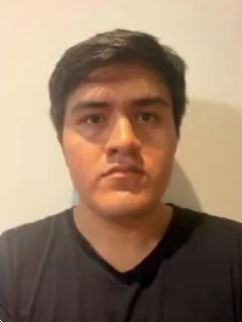
\includegraphics[width=\linewidth]{images/foto-original.png}\\[2pt]\footnotesize\emph{Foto original}
\end{minipage}\hfill
\begin{minipage}[t]{0.30\linewidth}
\centering
\includegraphics[width=\linewidth]{images/foto-recorte.png}\\[2pt]\footnotesize\emph{Recorte 512 × 512}
\end{minipage}\hfill
\begin{minipage}[t]{0.30\linewidth}
\centering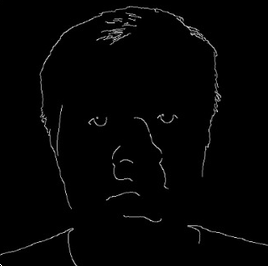
\includegraphics[width=\linewidth]{images/foto-canny.png}\\[2pt]\footnotesize\emph{Bordes Canny}
\end{minipage}
\caption{Ejemplo de foto en el pipeline de preprocesado: foto original, recorte de 512 × 512 px y mapa de bordes Canny que condiciona a ControlNet.}
\end{figure}

% ------------------------------ 4. Modelos generativos ------------------------------
\section*{4. Modelos generativos}

Cumplimos la condición de implementar dos de los tres niveles del enunciado, de modo que funcionen como alternativas y el usuario elija desde la interfaz:

\begin{itemize}
\item \textbf{Nivel intermedio (enfoque principal).} Usa Stable Diffusion 1.5 (\texttt{stable-diffusion-v1-5/stable-diffusion} \texttt{-v1-5}) con ControlNet Canny (\texttt{lllyasviel/control\_v11p\_sd15\_canny}) en modo img2img. La foto se usa como punto de partida y los bordes Canny se usan como condición estructural, con una escala de condicionamiento de 0,85.
\item \textbf{Nivel básico (alternativa).} Usa Stable Diffusion 1.5 en modo img2img sin ControlNet (en el sentido de SDEdit). Comparte la UNet, el VAE y el codificador de texto con el nivel intermedio, así que no ocupa memoria adicional en la GPU.
\end{itemize}

\textbf{Parámetros comunes:} 25 pasos con el planificador UniPC, \emph{guidance scale} de 7,0 a 8,0 y \emph{strength} de 0,40 a 0,50 según el estilo. Para comparar entre métodos se usan semillas fijas (1234 más el índice de la variación).

Los textos de condicionamiento están en inglés, que es el idioma de entrenamiento del codificador CLIP, y miden entre 35 y 43 tokens, por debajo del límite de 77. El texto libre del usuario se antepone a la descripción del estilo, después de pasar el filtro ético.

\textbf{Personalización con LoRA.} Por las restricciones de acceso al clúster Khipu, el docente indicó priorizar la personalización con LoRA en plataformas gratuitas. Integramos el LoRA público \texttt{OedoSoldier/detail-tweaker-lora} (\texttt{add\_detail.safetensors}, escala 0,6), que mejora el nivel de detalle en SD 1.5. LoRA congela los pesos del modelo y aprende una actualización de bajo rango, $\Delta W = BA$, sobre las capas de atención. Por eso se carga en segundos y casi no ocupa memoria. El adaptador se puede activar o desactivar en cada petición para comparar resultados.

En la primera corrida en Colab el LoRA no cargó por un conflicto de versiones de torchao: Colab trae preinstalada la versión 0.10.0 y la librería \texttt{peft} exige una superior a 0.16.0. El notebook final desinstala \texttt{torchao} antes de cargar los modelos. Con ese cambio, en la segunda corrida el LoRA cargó (384 capas en la UNet y 144 en el codificador de texto) y se aplicó a todas las variaciones. La sección 7 compara ambas corridas.

\textbf{Despliegue.} El notebook \texttt{controlnet\_portrait\_pipeline.ipynb} se ejecuta con ``Ejecutar todas''. Instala dependencias, sube la foto, genera los experimentos de la sección 7, descarga un zip con las imágenes y métricas, y deja el servidor GPU publicado con una URL de Cloudflare que se pega en la interfaz.

% ------------------------------ 5. Interfaz e interacción ------------------------------
\section*{5. Interfaz e interacción humano–IA}

\begin{figure}[H]
    \centering
    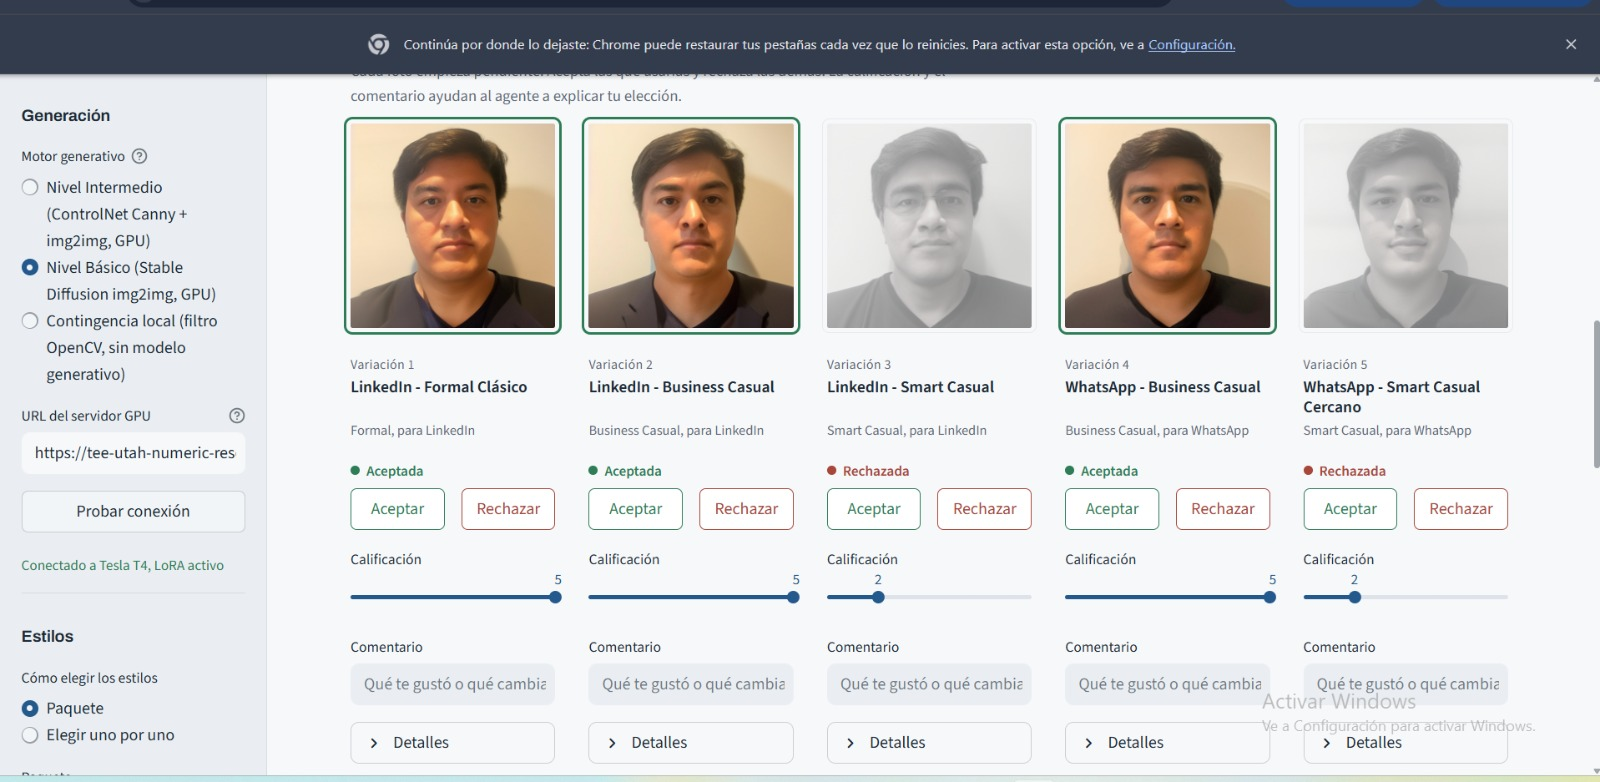
\includegraphics[width=\linewidth]{images/cap3.jpeg}
    \caption{Paso 2 de la interfaz, conectada a la GPU de Colab: las variaciones aceptadas quedan enmarcadas en verde y las rechazadas pasan a gris, cada una con su calificación y comentario.}
\end{figure}

La interfaz sigue el flujo de la sección 1:

\begin{itemize}
\item \textbf{Selección de estilos:} la barra lateral permite elegir el motor (intermedio, básico o contingencia local), un paquete temático o una selección manual de estilos, y escribir un ajuste de vestimenta en texto libre.
\item \textbf{Filtro inmediato:} el filtro ético revisa ese texto mientras se escribe y bloquea la solicitud con un mensaje explícito (Anexo B).
\item \textbf{Decisión pendiente:} las variaciones se muestran juntas, como una hoja de contactos de fotografía, cada una con su estilo y en estado \textbf{Pendiente}. El sistema no asume ninguna aprobación hasta que el usuario vota.
\item \textbf{Retroalimentación por imagen:} botones \emph{Aceptar} y \emph{Rechazar}, una calificación de 1 a 5 y un comentario. Al votar, la variación aceptada queda enmarcada en verde y la rechazada pasa a gris, de modo que la selección se ve de un vistazo.
\item \textbf{Transparencia:} antes de generar, la interfaz muestra el recorte de 512 × 512 px y los bordes Canny que guiarán al modelo.
\end{itemize}

Cada acción se guarda de inmediato en \texttt{data/processed/user\_decisions.json}, que se puede descargar desde la pantalla. Cada registro incluye la variación, el estilo, la decisión, la calificación, el comentario, el motor usado y la latencia medida (Anexo C). Cada lote generado se guarda en \texttt{data/processed/generated/} con la entrada, los bordes, las cinco imágenes y sus tiempos. La barra lateral también permite asociar las decisiones a un código anónimo de participante y cerrar la sesión en un archivo independiente.

Completar el ciclo toma nueve acciones: subir la foto, elegir el paquete, generar, votar cinco veces y pedir la explicación. Con la GPU de Colab, el tiempo de espera es de 25 a 35 s por lote de cinco imágenes, más 4 a 20 s del agente.

% ------------------------------ 6. Agente explicador ------------------------------
\section*{6. Agente explicador}

El agente (Figura 4) recibe el registro de decisiones y produce primero una lista determinista de las variaciones aceptadas y rechazadas, con su calificación y comentario. Esa lista proviene del JSON y no del modelo de lenguaje, lo que garantiza que el requisito central del enunciado se cumpla siempre. Después pide al modelo de lenguaje una explicación con cuatro secciones: conteos, cada aceptada con su motivo, cada rechazada con su motivo y recomendaciones para la siguiente generación. Las instrucciones exigen usar solo los datos entregados y no omitir ninguna variación.

\begin{figure}[H]
    \centering
    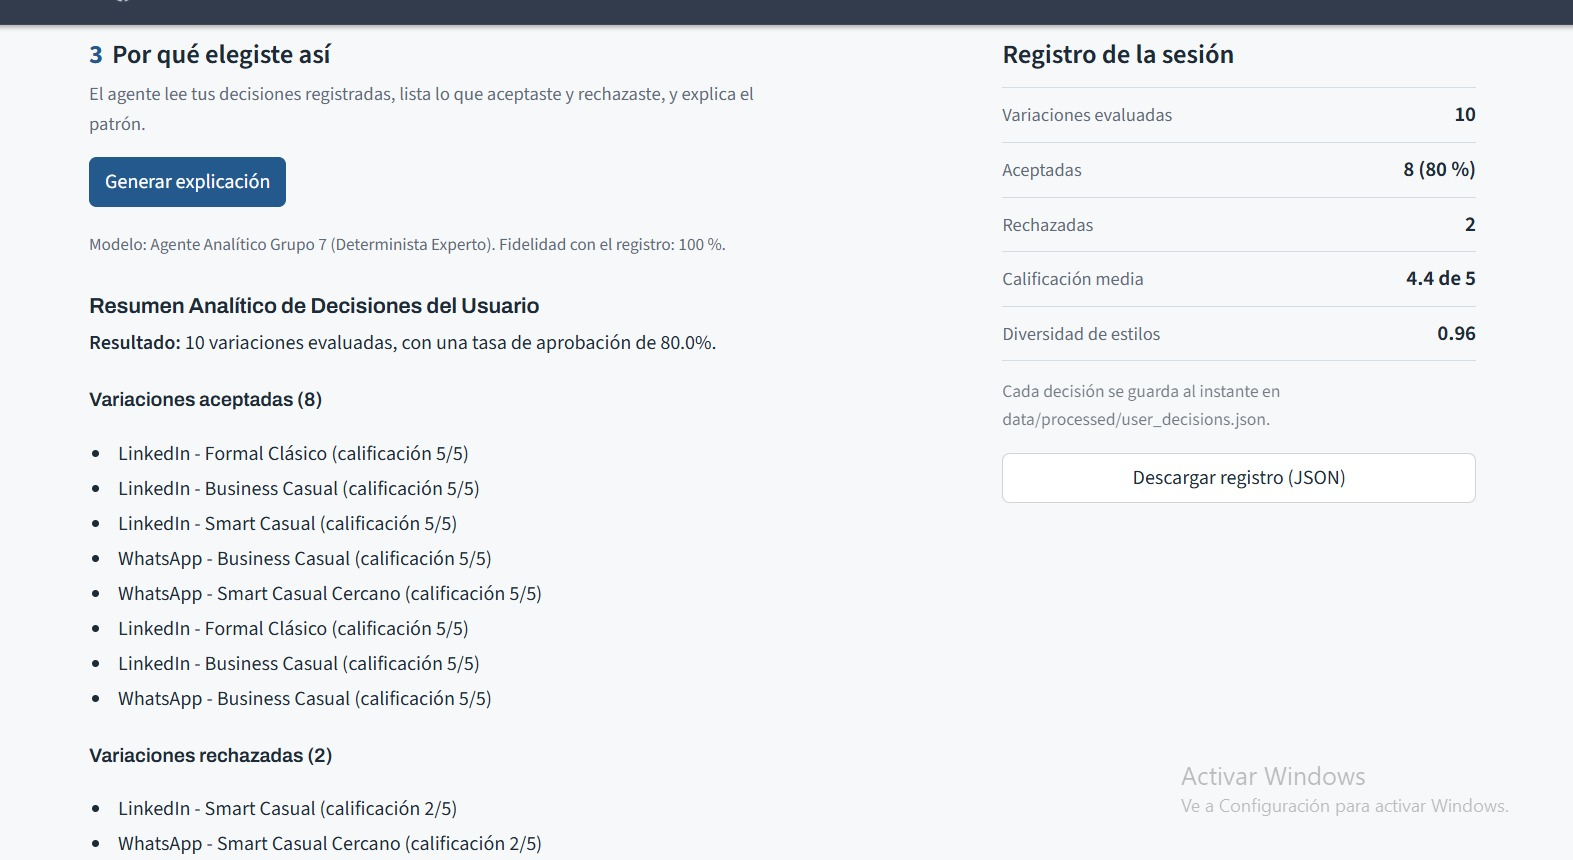
\includegraphics[width=\linewidth]{images/cap4.jpeg}
    \caption{Paso 3 de la interfaz: explicación generada por Gemini 3.5 Flash Lite para las decisiones de la Figura 3, con su fidelidad calculada y el registro de la sesión.}
\end{figure}

Siguiendo la sugerencia de comparar más de un modelo de lenguaje, el agente ofrece tres opciones:

\begin{itemize}
\item \textbf{Gemini 3.5 Flash Lite} (API de Google), con una cadena de respaldo: Gemini 3.1 Flash Lite, Flash Lite Latest y Gemini 3.8 Flash. Reintenta ante errores 429 y 503 y pasa al siguiente modelo si uno no responde en 25 s.
\item \textbf{GPT-4o-mini} (API de OpenAI). Está implementado, pero no lo evaluamos por no contar con una clave de API.
\item \textbf{Agente de reglas} sin conexión, que agrega estadísticas de plataforma, formalidad e iluminación.
\end{itemize}

Si ningún modelo responde, el sistema usa el agente de reglas y lo informa en pantalla junto con el motivo.

\textbf{Fidelidad.} \texttt{evaluator.py} comprueba que cada título votado aparezca asociado a su decisión correcta y que estén los tres conteos (total, aceptadas y rechazadas):

\[
\text{Fidelidad} = \frac{\text{comprobaciones correctas}}{\text{número de variaciones votadas} + 3}
\]

La métrica se calcula sobre cada explicación y se muestra al usuario. No es una constante.

% ------------------------------ 7. Evaluación y resultados ------------------------------
\section*{7. Evaluación y resultados}

Todas las mediciones se hicieron en una Tesla T4, con la foto B, el paquete de 5 variaciones, 25 pasos y semillas fijas. Hicimos dos corridas con la misma configuración: la primera sin LoRA, por el conflicto descrito en la sección 4, y la segunda con LoRA. Los scripts y los datos crudos están en \texttt{material\_apoyo/informe/}.

% Tabla 2: Comparación de métricas
\begin{table}[htbp]
\centering
\caption{Comparación de métricas entre configuraciones del motor generativo.}
\label{tab:metricas}
\footnotesize
\renewcommand{\arraystretch}{1.25}
\resizebox{\linewidth}{!}{%
\begin{tabular}{@{} p{1.65cm} p{2.35cm} >{\centering\arraybackslash}p{1.05cm} >{\centering\arraybackslash}p{1.05cm} >{\centering\arraybackslash}p{1.05cm} >{\centering\arraybackslash}p{1.05cm} @{}}
\toprule
\textbf{Métrica} & \textbf{Definición} & \textbf{Interm.\ sin LoRA} & \textbf{Interm.\ con LoRA} & \textbf{Básico sin LoRA} & \textbf{Básico con LoRA} \\
\midrule
Latencia en la GPU & Segundos por imagen & 2,61 s & 2,88 s & 1,96 s & 2,28 s \\
\addlinespace
Diversidad visual & Diferencia media absoluta entre pares de imágenes (0--1) & 0,036 & 0,038 & 0,040 & 0,041 \\
\addlinespace
Detalle & Varianza del Laplaciano (entrada: 86,9) & 101,8 & 102,5 & 100,4 & 101,7 \\
\addlinespace
Cambio de luminosidad de la piel & $\Delta L^\star$ medio en el centro de la cara (escala 0--100) & $-0,39$ & $-0,43$ & $-0,35$ & $-0,44$ \\
\addlinespace
Diferencia de color de la piel & $\Delta E$ medio en el centro de la cara & 1,87 & 1,95 & 2,14 & 2,30 \\
\bottomrule
\end{tabular}%
}
\end{table}

En el registro de métricas se activó una marca NSFW en la variación \texttt{nivel\_basico\_img2img/var3\_linkedin\_smart\_casual.png}, mientras que el resto de las imágenes del lote figuraron sin marca. Conviene revisar si correspondió a un falso positivo del filtro de seguridad de Stable Diffusion sobre el recorte facial.

\begin{figure}[H]
    \centering
    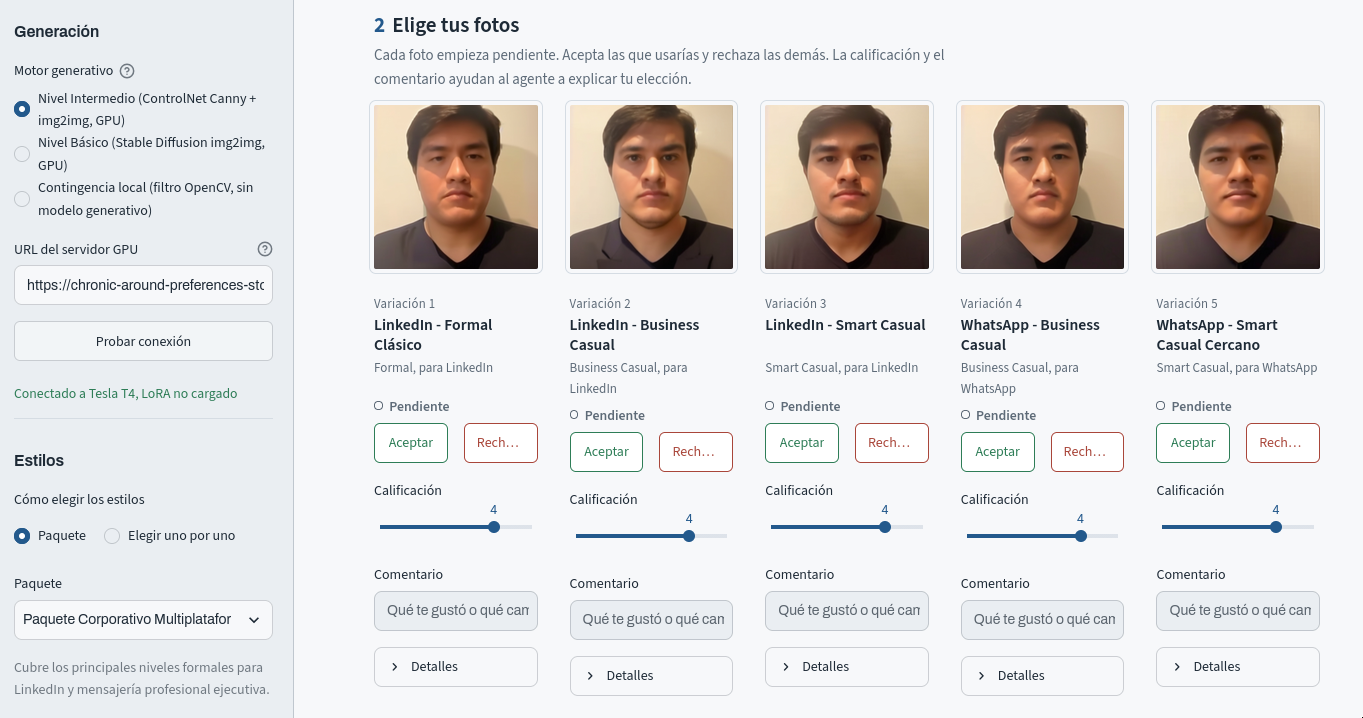
\includegraphics[width=\linewidth]{images/sin-lora.png}
    \caption{Nivel intermedio (ControlNet Canny + img2img) sin LoRA: las 5 variaciones del paquete corporativo. Con LoRA el resultado es prácticamente igual. El nivel básico se muestra en el Anexo A.}
\end{figure}

\textbf{Calidad y diversidad.}

\begin{itemize}
\item \textbf{Calidad:} las imágenes son fotorrealistas, sin artefactos graves ni deformaciones faciales, y conservan pose, encuadre y expresión.
\item \textbf{Diversidad baja:} con \emph{strength} entre 0,42 y 0,48 la ropa cambia poco. El color y el corte de la polera original se mantienen. Solo ``Business Casual'' muestra un blazer y ``Smart Casual Cercano'' agrega un cuello de polo; en ``Formal Clásico'' no aparece el terno. La diferencia media entre variaciones (0,036 a 0,040) confirma que se parecen mucho entre sí.
\item \textbf{Comparación entre métodos:} con la misma semilla, los dos niveles producen resultados muy parecidos. Con esta intensidad, la imagen de partida pesa más que el condicionamiento de ControlNet, y el nivel básico es entre un 21\% y un 25\% más rápido.
\end{itemize}

\textbf{Intensidad frente a identidad.}

\begin{itemize}
\item \textbf{Ropa:} el terno aparece a partir de 0,60.
\item \textbf{Pelo:} al aumentar \emph{strength} a 0,60 y 0,75—o en estilos como \emph{LinkedIn -- Smart Casual} y \emph{WhatsApp -- Business Casual}—se aprecia variación en la textura del cabello y arrastre cromático asociado a la descripción del estilo, reflejando el compromiso entre modificar la vestimenta y conservar la identidad.
\item \textbf{Rasgos:} con 0,60 y 0,75 también cambian la nariz y los labios, y la persona deja de ser reconocible.
\item \textbf{Color del terno:} en ``Formal Clásico'', el ``azul marino'' del texto tiñe el pelo.
\item \textbf{Piel:} el cambio es pequeño ($\DurL$ medio de -0,4 en el centro de la cara; hasta -2,2 en la cara completa con \emph{strength} de 0,60 a 0,75). No es el efecto dominante.
\end{itemize}

Interpretamos el cambio de textura del pelo como un sesgo del modelo preentrenado, coherente con estudios que documentan estereotipos demográficos en SD (Bianchi et al., 2023; Luccioni et al., 2023), y lo tratamos como la limitación principal (sección 9).

\begin{figure}[H]
    \centering
    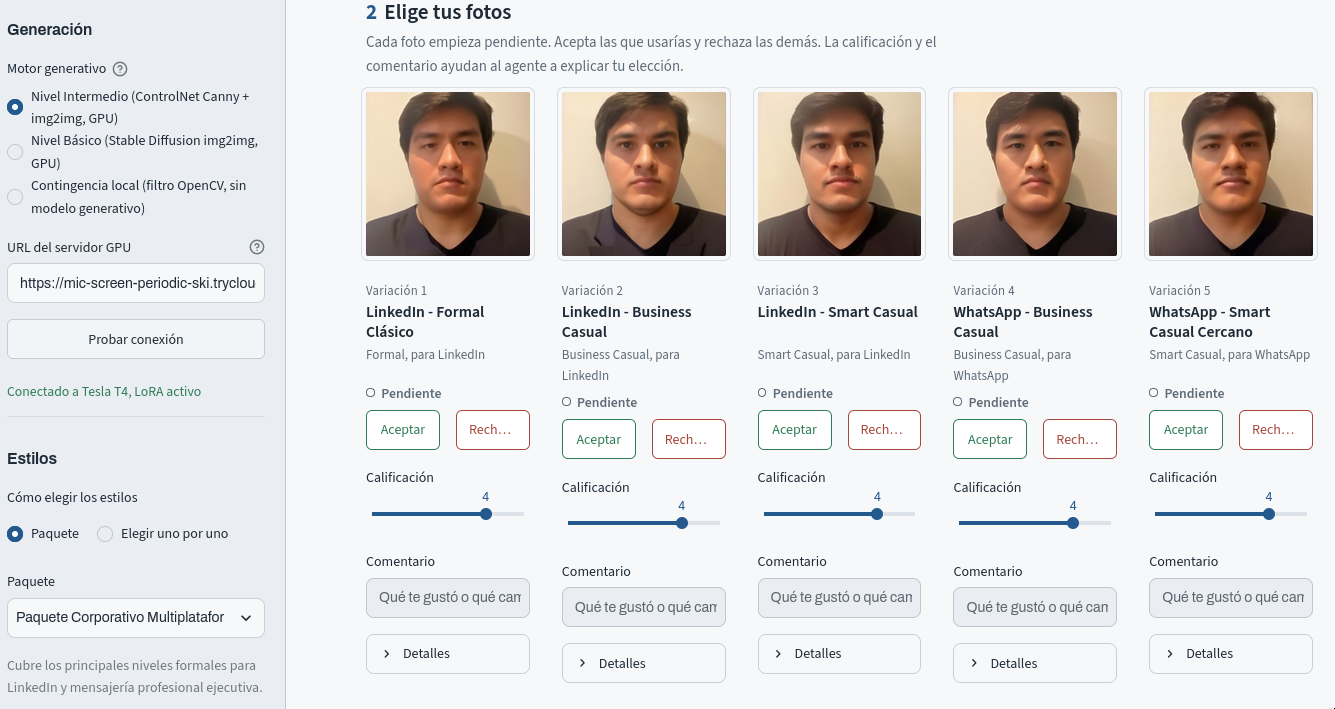
\includegraphics[width=\linewidth]{images/con-lora.png}
    \caption{Variaciones del paquete Corporativo Multiplataforma del lote Intermedio (\emph{strength} 0,42--0,48).}
\end{figure}

\textbf{Efecto del LoRA.} El adaptador funciona, pero su efecto es pequeño (Figura 7):

\begin{itemize}
\item \textbf{Detalle:} con el \emph{strength} de los estilos (0,42 a 0,48), aumenta entre 0,7\% y 1,3\%. A 0,60 aumenta 4,9\% (de 97,7 a 102,5).
\item \textbf{Diferencia de píxeles:} en promedio, 0,4\% a 0,7\% respecto de la imagen sin LoRA.
\item \textbf{Latencia:} suma unos 0,3 s por imagen.
\item \textbf{Identidad:} no cambia el compromiso entre ropa e identidad; el pelo se altera igual con y sin LoRA.
\end{itemize}

Es coherente con lo que es: un LoRA de detalle, usado con escala 0,6, que no aprendió un estilo corporativo.


\begin{figure}[H]
    \centering
    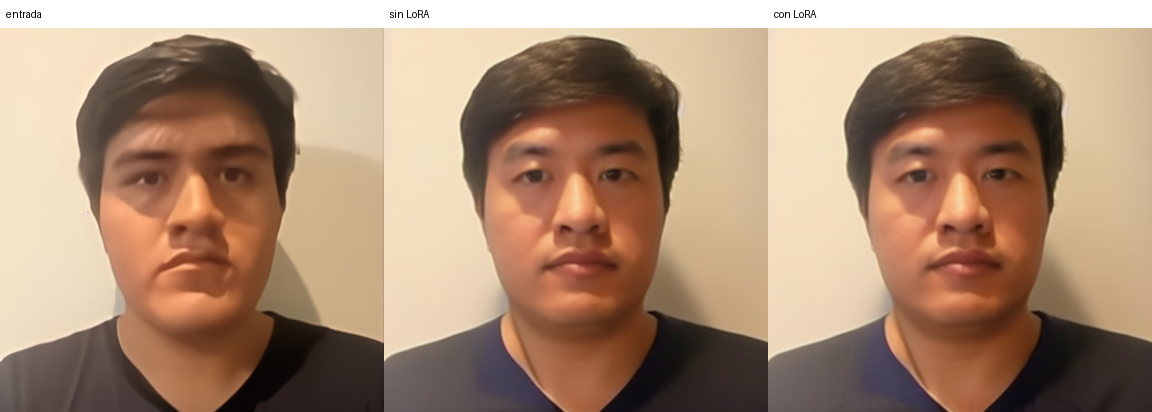
\includegraphics[width=\linewidth]{images/con-sin-lora.png}
    \caption{Estilo Formal Clásico con \emph{strength} 0,60 y la misma semilla: foto original, sin LoRA, con LoRA.}
\end{figure}


\textbf{Coherencia del agente.} Evaluamos el agente con 10 conjuntos de decisiones variadas sobre el paquete de 5 estilos:

\begin{table}[htbp]
\centering
\caption{Evaluación de fidelidad y latencia de los agentes explicadores.}
\label{tab:agentes}
\footnotesize
\renewcommand{\arraystretch}{1.25}
\resizebox{\linewidth}{!}{%
\begin{tabular}{@{} l >{\centering\arraybackslash}p{1.25cm} >{\centering\arraybackslash}p{1.55cm} >{\centering\arraybackslash}p{1.55cm} >{\centering\arraybackslash}p{1.85cm} @{}}
\toprule
\textbf{Agente} & \textbf{Corridas} & \textbf{Fidelidad media} & \textbf{Fidelidad mínima} & \textbf{Latencia media (máx.)} \\
\midrule
Gemini 3.5 Flash Lite & 10 & 100\% & 100\% & 11,9 s (19,9 s) \\
\addlinespace
Agente de reglas & 10 & 100\% & 100\% & $< 0,01\text{ s}$ \\
\bottomrule
\end{tabular}%
}
\end{table}

La primera versión de la métrica daba 93,8\% a Gemini. Al revisar los cinco casos con 87,5\%, encontramos que no eran errores del modelo, sino falsos negativos de la métrica ante frases como ``no fue aceptada a pesar de…''. Corregimos el manejo de negaciones y comprobamos que la métrica sigue detectando errores reales: con polaridad invertida, títulos omitidos o conteos incorrectos da entre 50\% y 67\%. En todas las corridas, Gemini listó las cinco variaciones con su decisión correcta y justificó cada una con la iluminación, el fondo y los comentarios del usuario, sin inventar preferencias.

% ------------------------------ 8. Iteraciones ------------------------------
\section*{8. Iteraciones guiadas por las pruebas}

\begin{table}[htbp]
\centering
\caption{Incidencias identificadas durante las pruebas y ajustes realizados.}
\label{tab:pruebas-ajustes}
\footnotesize
\renewcommand{\arraystretch}{1.25}
\resizebox{\linewidth}{!}{%
\begin{tabular}{@{} p{1.85cm} p{3.275cm} p{3.275cm} @{}}
\toprule
\textbf{Prueba} & \textbf{Problema observado} & \textbf{Cambio realizado} \\
\midrule
Selfie muy cercana tomada desde abajo (foto A) & El detector facial no encontraba la cara & Reducción a 640 px, ecualización y dos clasificadores Haar \\
\addlinespace
Misma foto & El recorte no cabía, quedaba rectangular y al escalarlo achataba la cara & Recorte siempre cuadrado, limitado por los bordes de la foto \\
\addlinespace
Fotos de celular & La orientación EXIF no se aplicaba & Corrección de la orientación al subir la foto \\
\addlinespace
Agente con Gemini & Gemini 2.5 Flash no está disponible para cuentas nuevas; los modelos grandes respondían 503 o no respondían & Cadena de modelos \emph{lite} con reintentos: la latencia bajó de 68 s a 4--20 s \\
\addlinespace
Conexión con Colab & Cortes esporádicos del túnel de Cloudflare & Reintento automático de la petición \\
\addlinespace
Métrica de fidelidad & Falsos negativos con negaciones & Normalización de ``no fue aceptada / rechazada'' \\
\addlinespace
Filtro ético & Dejaba pasar variantes como ``s1n r0pa'' o ``shirtless'' & Normalización de números usados como letras y términos nuevos \\
\addlinespace
Primera corrida en Colab & El LoRA no cargó por el conflicto con \texttt{torchao} & Desinstalación de \texttt{torchao} en el notebook; en la segunda corrida el LoRA carga \\
\bottomrule
\end{tabular}%
}
\end{table}

% ------------------------------ 9. Limitaciones y trabajo futuro ------------------------------
\section*{9. Limitaciones y trabajo futuro}

\begin{enumerate}
\item \textbf{Identidad frente a vestimenta.} El img2img aplicado a toda la imagen obliga a elegir entre conservar la identidad (\emph{strength} bajo) y cambiar la ropa (\emph{strength} alto). La mejora propuesta es usar \emph{inpainting} con una máscara facial, que conserva los píxeles reales de la cara y el pelo y regenera solo la ropa y el fondo (Lugmayr et al., 2022), con un \emph{strength} de 0,75 o más.
\item \textbf{Influencia de los bordes Canny.} Los bordes fijan también el cuello de la polera original, lo que dificulta dibujar un cuello de camisa. Una alternativa es atenuar los bordes en la zona del torso.
\item \textbf{Alcance del LoRA.} El LoRA público mejora poco el detalle y no aporta un estilo de retrato corporativo. Un LoRA entrenado en Colab con retratos ejecutivos de licencia libre permitiría personalizar de verdad la vestimenta y la iluminación.
\item \textbf{Alcance de la métrica de fidelidad.} Supone que la explicación está organizada en secciones, con la decisión antes del título, que es el formato que se pide al modelo. No evalúa la calidad de las justificaciones.
\item \textbf{Infraestructura.} Las sesiones gratuitas de Colab expiran y el túnel cambia de URL en cada ejecución. Para la demostración se debe ejecutar el notebook poco antes.
\end{enumerate}

% ------------------------------ 10. Consideraciones éticas ------------------------------
\section*{10. Consideraciones éticas}

\textbf{Manipulación de identidad.} Un sistema que modifica retratos puede usarse para suplantar a otra persona o para presentarse de forma engañosa. Lo limitamos de tres formas: el caso de uso es la propia foto del usuario, las variaciones son estilos profesionales acotados y la interfaz no ofrece edición libre de rasgos. Por eso la interfaz deja la decisión final en manos del usuario y no publica nada de forma automática. Nuestros resultados muestran que el modelo puede alterar rasgos sin pedirlo.

\textbf{Sesgo.} El cambio de textura del pelo y la filtración de colores del texto al pelo son sesgos heredados del preentrenamiento con datos web. Afectan más a personas cuyos rasgos están menos representados en esos datos. Lo reportamos en lugar de ocultarlo y la mejora de la sección 9 lo ataca directamente.

\textbf{Guardrails implementados:}

\begin{itemize}
\item Filtro léxico preventivo con normalización de tildes y de números usados como letras. Bloquea antes de usar la GPU y muestra la categoría de la infracción.
\item El filtro de contenido de Stable Diffusion se mantiene activo y su resultado se registra en cada imagen.
\item El prompt negativo excluye desnudez y deformaciones.
\end{itemize}

\textbf{Privacidad.} Las fotos y decisiones se guardan en \texttt{data/processed/}, excluida del repositorio por \texttt{.gitignore}. La clave de API se lee de un archivo \texttt{.env} que no se versiona. El código de participante es anónimo. Las fotos de este informe son de un integrante del equipo y se usan con su consentimiento.

\textbf{Propiedad intelectual.} SD 1.5 se distribuye bajo la licencia CreativeML OpenRAIL-M y ControlNet bajo OpenRAIL. Ambas permiten el uso con restricciones de uso responsable. El LoRA es de un tercero y se cita como tal. La autoría de imágenes generadas a partir de la foto de una persona y de un modelo entrenado con obras de terceros es una pregunta abierta que el usuario debe considerar antes de publicar.

% ------------------------------ 11. Conclusiones ------------------------------
\section*{11. Conclusiones}

El sistema cumple el ciclo del enunciado de extremo a extremo:

\begin{itemize}
\item genera cinco variaciones por foto con dos métodos en una GPU gratuita;
\item registra decisiones estructuradas por imagen;
\item produce una explicación que lista explícitamente lo aceptado y lo rechazado, con 100\% de fidelidad medida en 10 corridas.
\end{itemize}

La evaluación cuantitativa mostró que el control de la ropa y la conservación de la identidad compiten cuando el img2img se aplica a toda la imagen. Este hallazgo, más que las cifras de latencia, es el aporte principal: indica que el siguiente paso es conservar la cara por máscara y no aumentar la intensidad del modelo.

% ------------------------------ Bibliografía ------------------------------
\section*{Bibliografía}

\begin{enumerate}
\item Amershi, S., Weld, D., Vorvoreanu, M., Fergus, A., ... y Horvitz, E. (2019). Guidelines for human-AI interaction. \emph{Proceedings of the 2019 CHI Conference on Human Factors in Computing Systems}, 1–13.
\item Bianchi, F., Kalluri, P., Durmus, E., Ladhak, F., Cheng, M., Nozza, D., ... y Caliskan, A. (2023). Easily accessible text-to-image generation amplifies demographic stereotypes at large scale. \emph{Proceedings of the 2023 ACM Conference on Fairness, Accountability, and Transparency}, 1493–1504.
\item Brown, T. (2008). Design thinking. \emph{Harvard Business Review}, 86(6), 84–92.
\item Canny, J. (1986). A computational approach to edge detection. \emph{IEEE Transactions on Pattern Analysis and Machine Intelligence}, 8(6), 679–698.
\item Ho, J., Jain, A. y Abbeel, P. (2020). Denoising diffusion probabilistic models. \emph{Advances in Neural Information Processing Systems}, 33, 6840–6851.
\item Hu, E. J., Shen, Y., Wallis, P., Allen-Zhu, Z., Li, Y., Wang, S., Wang, L. y Chen, W. (2022). LoRA: Low-rank adaptation of large language models. \emph{International Conference on Learning Representations}.
\item Luccioni, A. S., Akiki, C., Mitchell, M. y Jernite, Y. (2023). Stable bias: Evaluating societal representations in diffusion models. \emph{Advances in Neural Information Processing Systems}, 36 (Datasets and Benchmarks Track).
\item Lugmayr, A., Danelljan, M., Romero, A., Yu, F., Timofte, R. y Van Gool, L. (2022). RePaint: Inpainting using denoising diffusion probabilistic models. \emph{Proceedings of the IEEE/CVF Conference on Computer Vision and Pattern Recognition}, 11461–11470.
\item Meng, C., He, Y., Song, Y., Song, J., Wu, J., Zhu, J.-Y. y Ermon, S. (2022). SDEdit: Guided image synthesis and editing with stochastic differential equations. ICLR.
\item Rombach, R., Blattmann, A., Lorenz, D., Esser, P. y Ommer, B. (2022). High-resolution image synthesis with latent diffusion models. \emph{Proceedings of the IEEE/CVF Conference on Computer Vision and Pattern Recognition}, 10684–10695.
\item Schuhmann, C., Beaumont, R., Vencu, R., Gordon, C., Wightman, R., Cherti, M., ... y Jitsev, J. (2022). LAION-5B: An open large-scale dataset for training next generation text-image models. \emph{Advances in Neural Information Processing Systems}, 35 (Datasets and Benchmarks Track).
\item Viola, P. y Jones, M. (2001). Rapid object detection using a boosted cascade of simple features. \emph{Proceedings of the 2001 IEEE Computer Society Conference on Computer Vision and Pattern Recognition}, 511–518.
\item Zhang, L., Rao, A. y Agrawala, M. (2023). Adding conditional control to text-to-image diffusion models. \emph{Proceedings of the IEEE/CVF International Conference on Computer Vision}, 3836–3847.
\end{enumerate}

Recursos de software: Hugging Face Diffusers y PEFT; Streamlit; FastAPI; OpenCV; API de Google Gemini; LoRA \texttt{OedoSoldier/detail-tweaker-lora} (Hugging Face).

% ------------------------------ Anexos ------------------------------
\section*{Anexo A. Ejemplos de variaciones}

\begin{figure}[H]
    \centering
    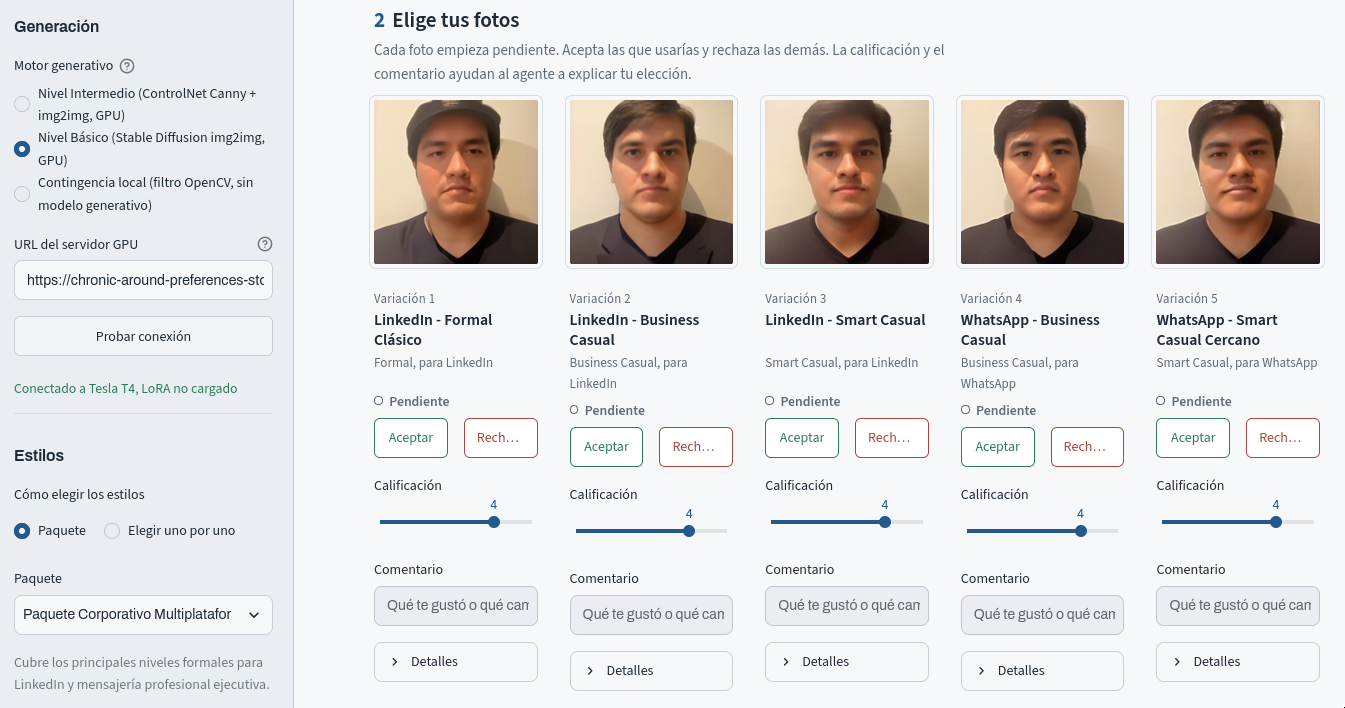
\includegraphics[width=\linewidth]{images/sin-lora-basico.png}
    \caption{Resultados disponibles (lote Intermedio); re-ejecutar el notebook en Colab para obtener las variaciones del Nivel Básico. Con la misma foto y las mismas semillas que la Figura 5.)}
\end{figure}

\textbf{Catálogo de estilos.} El paquete evaluado es ``Corporativo Multiplataforma'', de 5 variaciones.

\begin{table}[htbp]
\centering
\caption{Parámetros de generación y descripciones por estilo y red.}
\label{tab:estilos}
\footnotesize
\renewcommand{\arraystretch}{1.25}
\resizebox{\linewidth}{!}{%
\begin{tabular}{@{} p{2.0cm} p{1.25cm} p{3.85cm} >{\centering\arraybackslash}p{0.85cm} >{\centering\arraybackslash}p{0.85cm} @{}}
\toprule
\textbf{Estilo} & \textbf{Red} & \textbf{Vestimenta (texto para el modelo, resumido)} & \textbf{Strength} & \textbf{Guidance} \\
\midrule
LinkedIn -- Formal Clásico & LinkedIn & Navy blue business suit, white shirt, tie & 0,42 & 7,5 \\
\addlinespace
LinkedIn -- Business Casual & LinkedIn & Navy blazer, light blue open collar shirt & 0,45 & 7,5 \\
\addlinespace
LinkedIn -- Smart Casual & LinkedIn & Neat crew neck sweater & 0,48 & 7,0 \\
\addlinespace
WhatsApp -- Business Casual & WhatsApp & Casual blazer over a plain t-shirt & 0,43 & 7,2 \\
\addlinespace
WhatsApp -- Smart Casual Cercano & WhatsApp & Clean light polo shirt, bright daylight & 0,45 & 7,0 \\
\addlinespace
LinkedIn -- Black Tie & LinkedIn & Black tuxedo, bow tie & 0,40 & 8,0 \\
\addlinespace
GitHub -- Tech Casual & GitHub & Plain dark hoodie, monitors background & 0,46 & 7,5 \\
\addlinespace
Redes -- Creativo de Estudio & Redes & Modern tailored jacket, rim lighting & 0,50 & 8,0 \\
\bottomrule
\end{tabular}%
}
\end{table}

Todos los textos terminan con ``professional headshot photo, sharp focus on face, realistic skin, 85mm lens'' y usan un prompt negativo que excluye deformaciones, ilustración, texto y desnudez.

\section*{Anexo B. Filtro ético en la interfaz}

\begin{figure}[H]
    \centering
    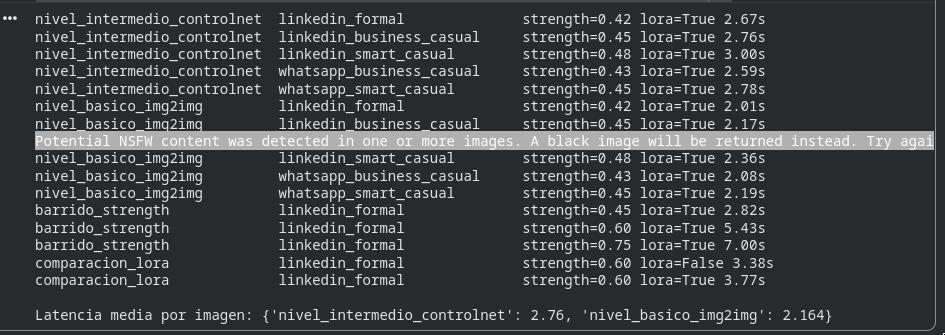
\includegraphics[width=\linewidth]{images/etico-1.png}
    \caption{Filtro ético bloqueando una imagen y su output en el backend en Google Colab.}
\end{figure}

\begin{figure}[H]
    \centering
    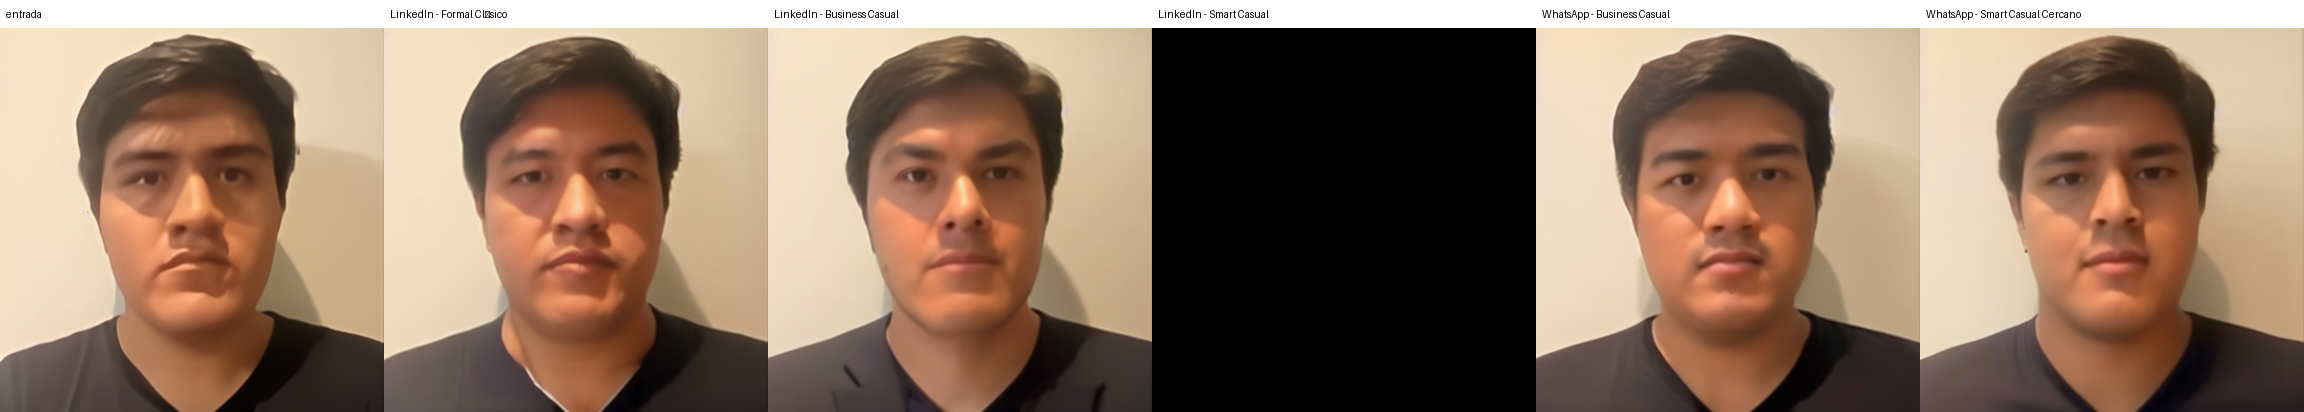
\includegraphics[width=\linewidth]{images/etico-2.png}
    \caption{Output recibido con una imagen bloqueada por el filtro ético: resultado es una imagen enteramente negra.}
\end{figure}


\section*{Anexo C. Registro de decisiones y salida del agente}

Registro real de la sesión de la Figura 3 (\texttt{user\_decisions.json}, primera de cinco entradas):

\begin{lstlisting}[
  language=json,
  basicstyle=\ttfamily\scriptsize,
  breaklines=true,
  breakatwhitespace=false,
  postbreak=\mbox{\textcolor{gray}{$\hookrightarrow$}\space},
  columns=fullflexible,
  keepspaces=true,
  frame=single,
  rulecolor=\color{black!30},
  xleftmargin=2pt,
  xrightmargin=2pt,
  literate={á}{{\'a}}1 {é}{{\'e}}1 {í}{{\'i}}1 {ó}{{\'o}}1 {ú}{{\'u}}1 {ñ}{{\~n}}1
           {Á}{{\'A}}1 {É}{{\'E}}1 {Í}{{\'I}}1 {Ó}{{\'O}}1 {Ú}{{\'U}}1 {Ñ}{{\~N}}1
]
{
  "variation_id": "gpu_var_linkedin_formal_55367",
  "preset_id": "linkedin_formal",
  "title": "LinkedIn - Formal Clásico",
  "platform": "LinkedIn",
  "formality": "Formal",
  "accepted": true,
  "rating": 4,
  "recommended_lighting": "Luz frontal difusa de tres puntos",
  "recommended_background": "Oficina corporativa moderna con bokeh suave",
  "user_notes": "Se ve serio, lo usaría en LinkedIn",
  "latency_seconds": 6.937,
  "engine_mode": "Nivel Intermedio (ControlNet Canny + img2img, GPU)"
}
\end{lstlisting}

Lista deterministica generada a partir de ese registro (sección 6):



\begin{lstlisting}[
  language=json,
  basicstyle=\ttfamily\scriptsize,
  breaklines=true,
  breakatwhitespace=false,
  postbreak=\mbox{\textcolor{gray}{$\hookrightarrow$}\space},
  columns=fullflexible,
  keepspaces=true,
  frame=single,
  rulecolor=\color{black!30},
  xleftmargin=2pt,
  xrightmargin=2pt,
  literate={á}{{\'a}}1 {é}{{\'e}}1 {í}{{\'i}}1 {ó}{{\'o}}1 {ú}{{\'u}}1 {ñ}{{\~n}}1
           {Á}{{\'A}}1 {É}{{\'E}}1 {Í}{{\'I}}1 {Ó}{{\'O}}1 {Ú}{{\'U}}1 {Ñ}{{\~N}}1
]
Resultado: 5 variaciones evaluadas, con una tasa de aprobación de 60.0%.
Variaciones aceptadas (3)
- LinkedIn - Formal Clásico (calificación 4/5) «Se ve serio, lo usaría en LinkedIn»
- LinkedIn - Smart Casual (calificación 4/5)
- WhatsApp - Business Casual (calificación 4/5) «Buena luz»
Variaciones rechazadas (2)
- LinkedIn - Business Casual (calificación 4/5) «El cuello de la polera no queda formal»
- WhatsApp - Smart Casual Cercano (calificación 4/5) «El pelo no se parece al mío»
\end{lstlisting}

En esta sesión de prueba no se movió el control de calificación, así que todas las variaciones quedaron con el valor inicial de 4.

\section*{Anexo D. Reproducibilidad}

\begin{enumerate}
\item \textbf{Servidor GPU.} Subir \texttt{notebooks/controlnet\_portrait\_pipeline} \texttt{.ipynb} a Google Colab, elegir GPU T4 y usar ``Ejecutar todas''. El notebook pide la foto, guarda los resultados en \texttt{resultados\_colab.zip} y publica el servidor con una URL \texttt{trycloudflare.com}.
\item \textbf{Interfaz.} En \texttt{Project-II}, ejecutar \texttt{uv sync} y luego ejecutar \texttt{run\_app.bat} o \texttt{run\_app.sh}. Pegar la URL del servidor y presionar ``Probar conexión''.
\item \textbf{Agente con Gemini.} Crear un archivo \texttt{.env} con la línea \texttt{GEMINI\_API\_KEY=...}.
\item \textbf{Métricas.} Ejecutar \texttt{material\_apoyo/} \texttt{informe/medir\_imagenes.py} (métricas de imagen) y \texttt{material\_apoyo/informe/} \texttt{evaluar\_agente.py 10} (fidelidad del agente). Los resultados se guardan en \texttt{material\_apoyo/informe/datos/}.
\end{enumerate}

Versiones probadas: Python 3.10 en local y 3.13 en Colab; en local, Diffusers 0.41, Transformers 5.20, PEFT 0.21 y Streamlit 1.65.

\end{document}
